\documentclass{article}\usepackage[]{graphicx}\usepackage[]{xcolor}
% maxwidth is the original width if it is less than linewidth
% otherwise use linewidth (to make sure the graphics do not exceed the margin)
\makeatletter
\def\maxwidth{ %
  \ifdim\Gin@nat@width>\linewidth
    \linewidth
  \else
    \Gin@nat@width
  \fi
}
\makeatother

\definecolor{fgcolor}{rgb}{0.345, 0.345, 0.345}
\newcommand{\hlnum}[1]{\textcolor[rgb]{0.686,0.059,0.569}{#1}}%
\newcommand{\hlsng}[1]{\textcolor[rgb]{0.192,0.494,0.8}{#1}}%
\newcommand{\hlcom}[1]{\textcolor[rgb]{0.678,0.584,0.686}{\textit{#1}}}%
\newcommand{\hlopt}[1]{\textcolor[rgb]{0,0,0}{#1}}%
\newcommand{\hldef}[1]{\textcolor[rgb]{0.345,0.345,0.345}{#1}}%
\newcommand{\hlkwa}[1]{\textcolor[rgb]{0.161,0.373,0.58}{\textbf{#1}}}%
\newcommand{\hlkwb}[1]{\textcolor[rgb]{0.69,0.353,0.396}{#1}}%
\newcommand{\hlkwc}[1]{\textcolor[rgb]{0.333,0.667,0.333}{#1}}%
\newcommand{\hlkwd}[1]{\textcolor[rgb]{0.737,0.353,0.396}{\textbf{#1}}}%
\let\hlipl\hlkwb

\usepackage{framed}
\makeatletter
\newenvironment{kframe}{%
 \def\at@end@of@kframe{}%
 \ifinner\ifhmode%
  \def\at@end@of@kframe{\end{minipage}}%
  \begin{minipage}{\columnwidth}%
 \fi\fi%
 \def\FrameCommand##1{\hskip\@totalleftmargin \hskip-\fboxsep
 \colorbox{shadecolor}{##1}\hskip-\fboxsep
     % There is no \\@totalrightmargin, so:
     \hskip-\linewidth \hskip-\@totalleftmargin \hskip\columnwidth}%
 \MakeFramed {\advance\hsize-\width
   \@totalleftmargin\z@ \linewidth\hsize
   \@setminipage}}%
 {\par\unskip\endMakeFramed%
 \at@end@of@kframe}
\makeatother

\definecolor{shadecolor}{rgb}{.97, .97, .97}
\definecolor{messagecolor}{rgb}{0, 0, 0}
\definecolor{warningcolor}{rgb}{1, 0, 1}
\definecolor{errorcolor}{rgb}{1, 0, 0}
\newenvironment{knitrout}{}{} % an empty environment to be redefined in TeX

\usepackage{alltt}
\usepackage{amsmath} %This allows me to use the align functionality.
                     %If you find yourself trying to replicate
                     %something you found online, ensure you're
                     %loading the necessary packages!
\usepackage{amsfonts}%Math font
\usepackage{graphicx}%For including graphics
\usepackage{hyperref}%For Hyperlinks
\usepackage[shortlabels]{enumitem}% For enumerated lists with labels specified
                                  % We had to run tlmgr_install("enumitem") in R
\hypersetup{colorlinks = true,citecolor=black} %set citations to have black (not green) color
\usepackage{natbib}        %For the bibliography
\setlength{\bibsep}{0pt plus 0.3ex}
\bibliographystyle{apalike}%For the bibliography
\usepackage[margin=0.50in]{geometry}
\usepackage{float}
\usepackage{multicol}

%fix for figures
\usepackage{caption}
\newenvironment{Figure}
  {\par\medskip\noindent\minipage{\linewidth}}
  {\endminipage\par\medskip}
\IfFileExists{upquote.sty}{\usepackage{upquote}}{}
\begin{document}

\vspace{-1in}
\title{Lab 03 -- MATH 240 -- Computational Statistics}

\author{
  Yuliia Heleveria \\
  MATH 240 Lab A  \\
  Mathematics  \\
  {\tt yheleveria@colgate.edu}
}

\date{02/25/2025}

\maketitle

\begin{multicols}{2}
\begin{abstract}
We want to analyze the contributions of The Front Bottoms, Manchester Orchestra, and All Get Out to their collaborative song ``Allentown'' using audio analysis. Therefore, we created a batch file to speed up data collection for audio features. The batch file contains 181 commands referring to 77 tracks by Manchester Orchestra, 61 by The Front Bottoms, 42 by All Get Out, and one collaborative track ``Allentown''. We analyzed musical characteristics of .WAV files from three bands, including valence, instrumental and acoustic features, emotional impact, loudness, and lyrics. We loaded and cleaned the data to perform analysis regarding characteristics of each band's tracks and their similarity with ``Allentown''. 
\end{abstract}

\noindent \textbf{Keywords:} Installing and using libraries; creating, cleaning, and merging data frames; looping structure; vectors and lists operations.

\section{Introduction}
``Allentown'' is a song released in 2018 by collaboration of The Front Bottoms and Manchester Orchestra. We would like to inspect which band made the most contribution to this song. We purchased all pre-``Allentown'' releases, totaling 181 tracks, including Allentown itself.
We use Essentia \citep{bogdanov2013essentia} to analyze, synthesize, and describe data about 181 songs to determine the musician who makes the most contribution to ``Allentown''. We analyze the style and characteristics of tracks, such as valence, arousal, emotions, and absence of voice or acoustic features, belonging to each band to determine stylistic features that resonate the most with ``Allentown''. 

This paper is structured as follows: In Section 2, we summarize the process of collecting, loading, and cleaning of data. Section 3 presents the outcome of data manipulation and analysis. In Section 4, we interpret the findings obtained by analyzing audio data given from 180 tracks of The Front Bottoms, Manchester Orchestra, and All Get Out compared to ``Allentown''.

\section{Methods}
For the purpose of data collection, we were given Essentia models \citep{alonso2020tensorflow} of 181 songs of interest. We used \texttt{stringr} package \citep{stringr} to create a batch file that creates command line prompts for each track. With the use of the batch file, we analyzed .WAV files for track characteristics, such as tempo in beats and average loudness.

Using \texttt{jsonlite} package for \texttt{R} \citep{jsonlite}, we extracted stylistic features of provided songs. We used \texttt{fromJSON()} to load JSON file containing music analysis into \texttt{R} and analyze average loudness, mean of spectral energy, dancebility, tempo in beats per minute, musical key, musical mode and duration of the track in seconds. We aslo used LIWC text analysis tool \citep{boyd2022development} to extract features that describe thoughts, feelings, and personality traits.

We loaded the data frame given from Essentia Model for 181 songs, including songs' valence, arousal, aggressiveness, acoustic and instrumental features. At the end, we merged three data frames and saved them to .csv files to combine output about lyrics and Essentia audio analysis. 

Using \texttt{tidyverse} package \citep{tidyverse}, we summarized data numerically for each feature of interest. We computed minimum, maximum, lower and upper fences for each feature for All Get Out, Manchester Orchestra, and The Front Bottoms to determine if ``Allentown'''s feature is within range or outlying for each band. Based of the statistical summaries, we computed visual aids of a table using \texttt{xtable} library \citep{xtable} and column plots using \texttt{tidyverse} to determine how ``Allentown'' differs of music of each band based on the count of how many features of ``Allentown'' are within range and out of range for each band..


\section{Results}
By creating a batch file, we significantly decreased the amount of time for data collection from multiple tracks at the same time using Essentia command line prompts. ``Allentown'' and its data was written separately into a different .csv file for data testing and determining the main band's contributions based on audio and lyrics analysis. The resulting .csv files contain data regarding spectral energy, tempo, dissonance, danceability, valence, happiness, tone, pronouns, etc. to derive conclusions of stylistic dominant features of each band in comparison of style with ``Allentown''. Three side-by-side column plots that demonstrate the count of features for each band that are outlying or that lie within range or out of range of ``Allentown'' demonstrate that Manchester Orchestra has the largest contribution to the collaborative track. Manchester Orchestra has the most musical features that lie within range of ``Allentown'' and the fewest features that are out of range. 

\section{Discussion}
We performed preliminary data analysis by creating \texttt{boxplot} that represent relation of data from ``Allentown'' in comparison to median values of the same data collected from three artists who participated in the song creation. 
Comparing the vertical line that represented ``Allentown'' in each plot, we cannot come to a conclusion of which artist has the closest audio style to ``Allentown''. In terms of overall loudness, ``Allentown'' is most similar to style of Manchester Orchestra, but ``Allentown'' has the overall word count of the median of The Front Bottoms tracks. In regard to aggressiveness, ``Allentown'' is the most similar to tracks by All Get Out. It is evident that three bands stylistically contribute to different audio featires of ``Allentown'', but more data analysis has to be performed to determine which band had the most contribution to creating the collaborative song.


%Code for creating an xtable and column plots

%code to process before graphs begin




%Code for creating boxplots to represent artist data






%Call the boxplots
\begin{figure}[H]
\begin{knitrout}\scriptsize
\definecolor{shadecolor}{rgb}{0.969, 0.969, 0.969}\color{fgcolor}
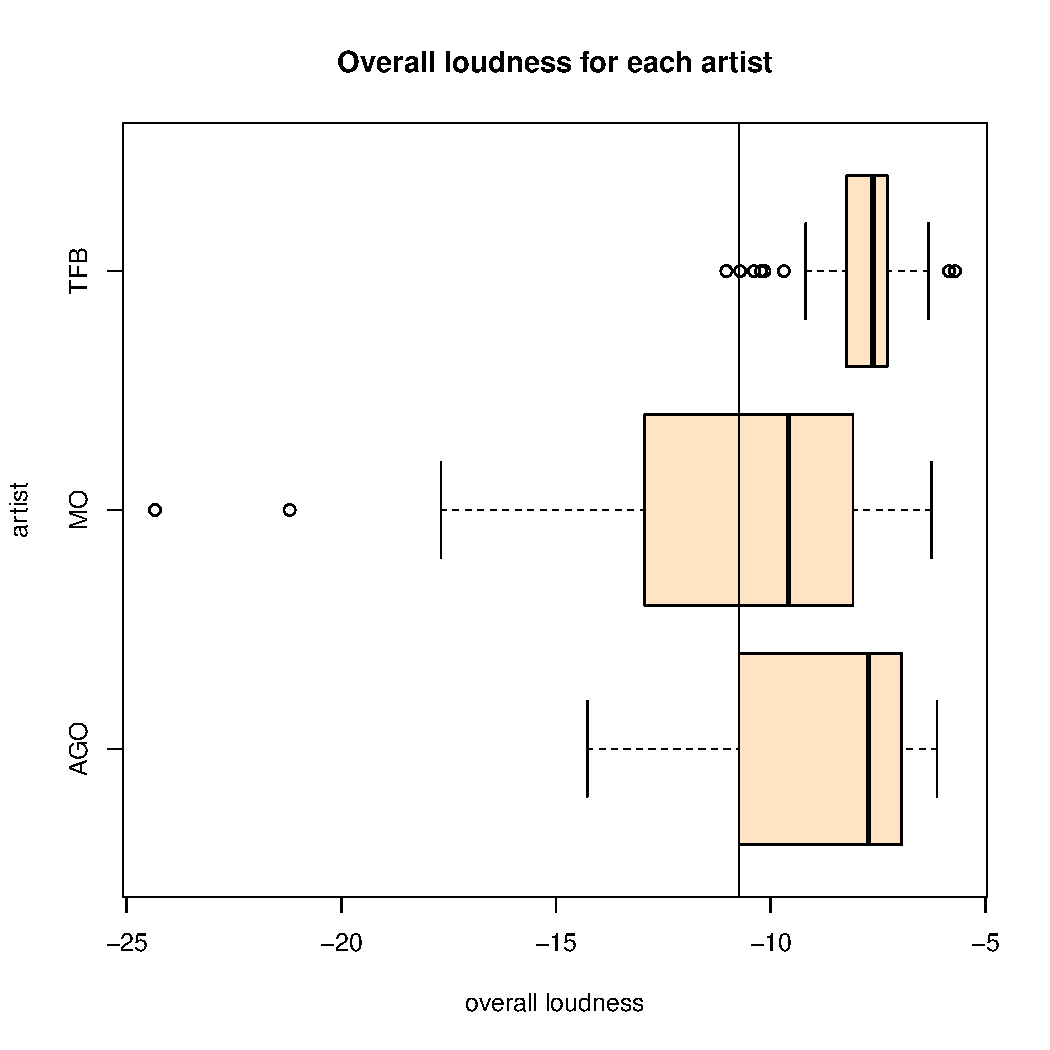
\includegraphics[width=\maxwidth]{figure/unnamed-chunk-3-1} 
\end{knitrout}
\caption{Vertical line represents ``Allentown''} \label{plot1}
\end{figure}

\begin{figure}[H]
\begin{knitrout}\scriptsize
\definecolor{shadecolor}{rgb}{0.969, 0.969, 0.969}\color{fgcolor}
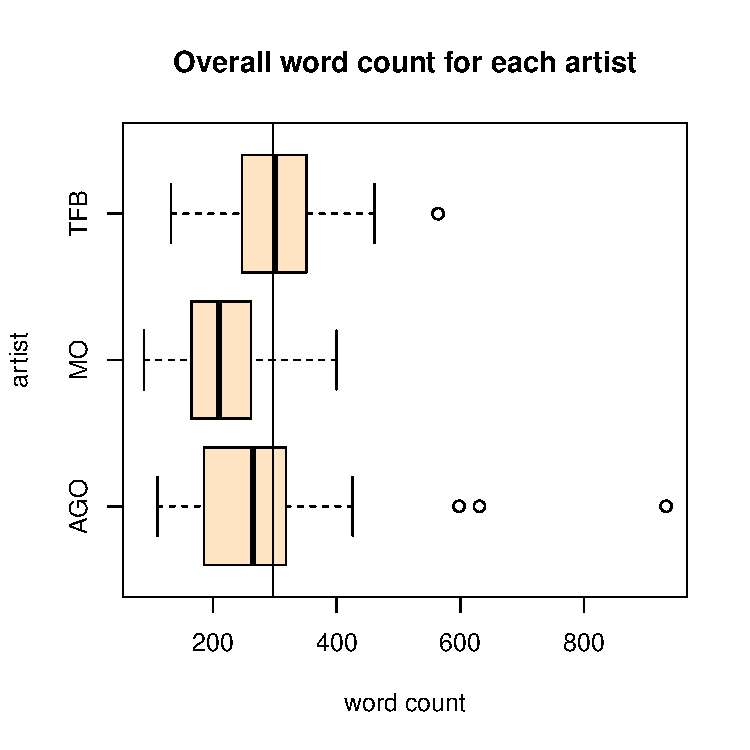
\includegraphics[width=\maxwidth]{figure/unnamed-chunk-4-1} 
\end{knitrout}
\caption{Vertical line represents ``Allentown''} \label{plot2}
\end{figure}

\begin{figure}[H]
\begin{knitrout}\scriptsize
\definecolor{shadecolor}{rgb}{0.969, 0.969, 0.969}\color{fgcolor}
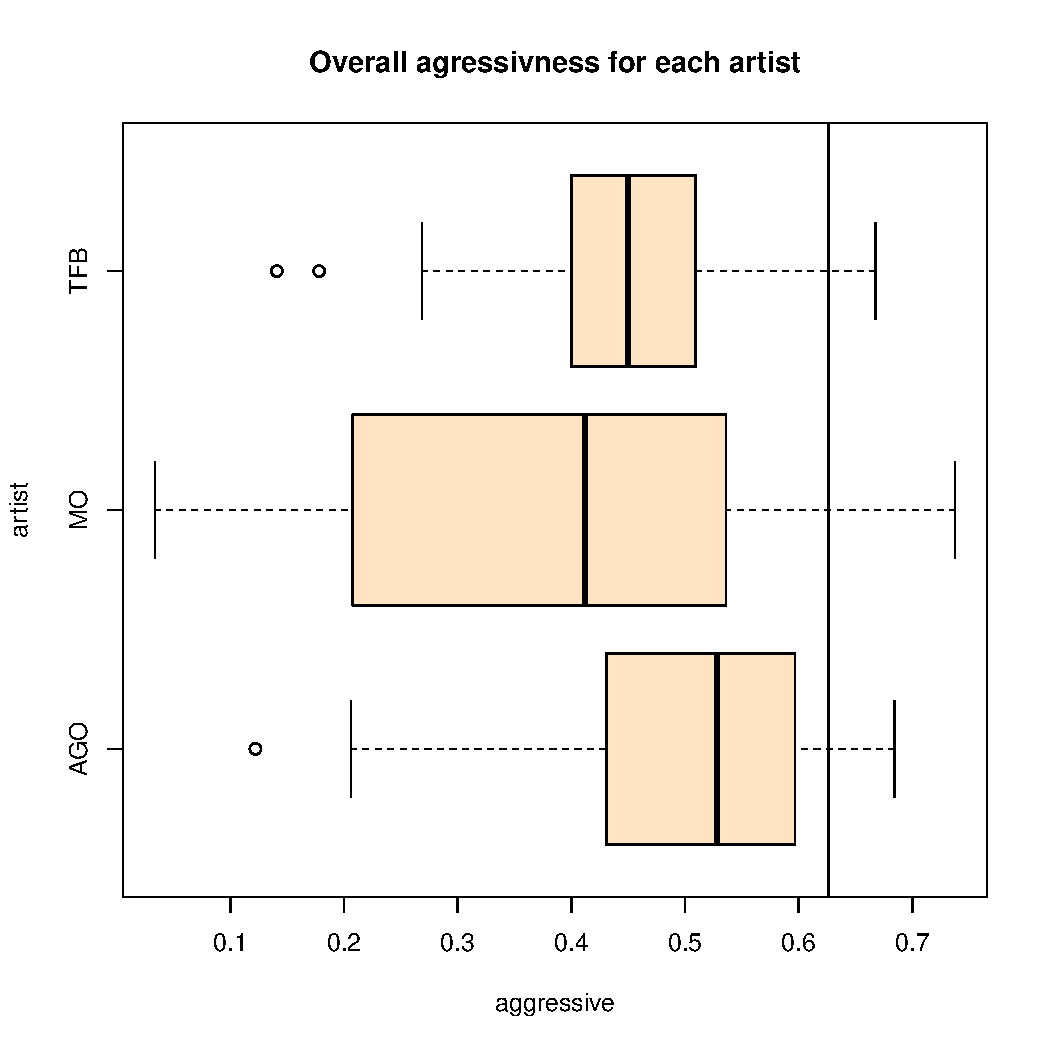
\includegraphics[width=\maxwidth]{figure/unnamed-chunk-5-1} 
\end{knitrout}
\caption{Vertical line represents ``Allentown''} \label{plot3}
\end{figure}

After analysis of all given features, it is evident that Manchester Orchestra has the most similar audio features to ``Allentown''. All Get Out has the second most similar audio features to ``Allentown'' because it has fewer out of range and more in range features than The Front Bottoms has (\ref{plot.allen}). However, Manchester Orchestra has significantly fewer out of range features than the other two bands, which leads us to conclude that Manchester Orchestra has the largest contributions to ``Allentown''.

%%%%%%%%%%%%%%%%%%%%%%%%%%%%%%%%%%%%%%%%%%%%%%%%%%%%%%%%%%%%%%%%%%%%%%%%%%%%%%%%
% Bibliography
%%%%%%%%%%%%%%%%%%%%%%%%%%%%%%%%%%%%%%%%%%%%%%%%%%%%%%%%%%%%%%%%%%%%%%%%%%%%%%%%
\vspace{2em}
\begin{tiny}
\bibliography{bib.bib}
\end{tiny}
\end{multicols}

%%%%%%%%%%%%%%%%%%%%%%%%%%%%%%%%%%%%%%%%%%%%%%%%%%%%%%%%%%%%%%%%%%%%%%%%%%%%%%%%
% Appendix
%%%%%%%%%%%%%%%%%%%%%%%%%%%%%%%%%%%%%%%%%%%%%%%%%%%%%%%%%%%%%%%%%%%%%%%%%%%%%%%%
\newpage
\onecolumn
\section{Appendix}
%creating an xtable
% latex table generated in R 4.4.2 by xtable 1.8-4 package
% Tue Feb 25 00:28:22 2025
\begin{table}[ht]
\centering
\begin{tabular}{|l|c|c|c|}
  \hline
Category & All.Get.Out & Manchester.Orchestra & The.Front.Bottoms \\ 
  \hline
Out of Range &  22 &   3 &  30 \\ 
  Outlying &  17 &  11 &  11 \\ 
  Within Range & 158 & 183 & 156 \\ 
   \hline
\end{tabular}
\caption{Comparison of Allentown's audio features with the range of band's features} 
\label{allentown.tab}
\end{table}


%creating column plots
\begin{figure}[H] \begin{center}
\begin{knitrout}
\definecolor{shadecolor}{rgb}{0.969, 0.969, 0.969}\color{fgcolor}
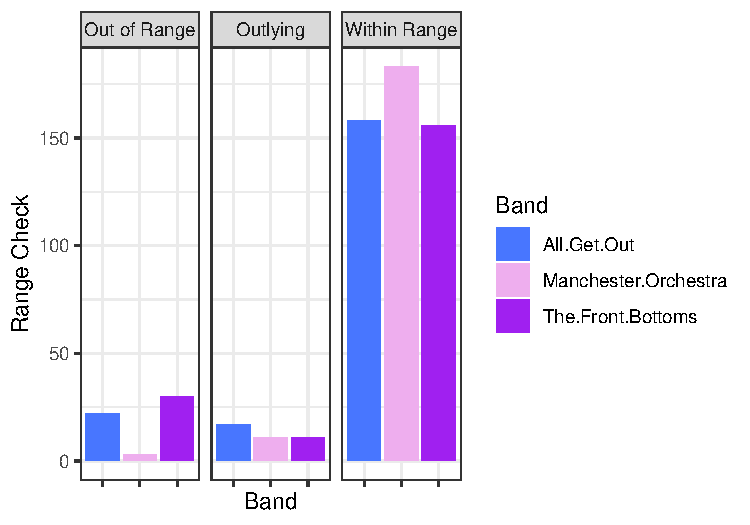
\includegraphics[width=\maxwidth]{figure/unnamed-chunk-7-1} 
\end{knitrout}
\caption{Comparison of Allentown's audio features with the range of band's features} \label{plot.allen}
\end{center}
\end{figure}


\end{document}
